\subsection{Geometry}
The two latest geometries are depicted in fig.~\ref{fig:geometry_v5} and fig.~\ref{fig:geometry_v6}. The patch boundaries and boundary conditions are indicated by the colored lines.

We also observe triple points within the computational domain. These are defined by material boundaries between air/vacuum, steel and the insulator.

\begin{center}
\begin{figure}[H]
   \begin{subfigure}{0.45\textwidth}
      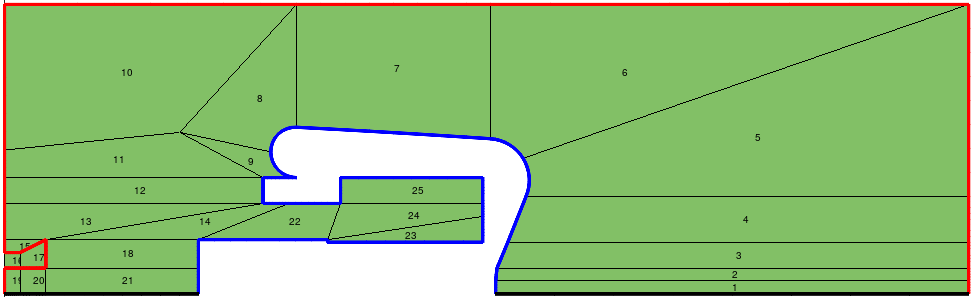
\includegraphics[width=\textwidth]{fig/geometry_v5}
      \caption{Version 5.}
      \label{fig:geometry_v5}
   \end{subfigure}
   \begin{subfigure}{0.45\textwidth}
      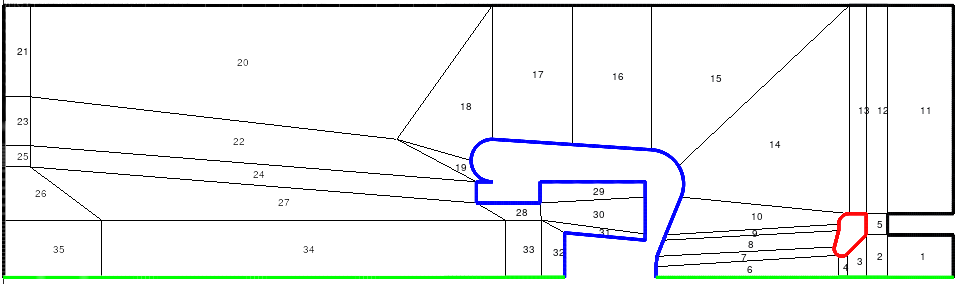
\includegraphics[width=\textwidth]{fig/geometry_v6}
      \caption{Version 6.}
      \label{fig:geometry_v6}
   \end{subfigure}
   % \caption{.}
\end{figure}
\end{center}

% \begin{center}
%    \begin{figure}[p]
%       \begin{tikzpicture}
\begin{axis}[
   scale only axis = true,
   width = 0.9\textwidth,
  axis equal,
  try min ticks=4,
  max space between ticks=1000pt,
  enlargelimits=true,
  colormap/Greens,
  point meta min = 0,
  point meta max = 2,
  x unit=m,
  y unit=m]

  \addplot[surf, shader=interp] table[point meta=\thisrow{c}]{figures/200kV/geometry/geometry_1.dat};

  \addplot[surf, shader=interp] table[point meta=\thisrow{c}]{figures/200kV/geometry/geometry_2.dat};

  \addplot[surf, shader=interp] table[point meta=\thisrow{c}]{figures/200kV/geometry/geometry_3.dat};

  \addplot[surf, shader=interp] table[point meta=\thisrow{c}]{figures/200kV/geometry/geometry_4.dat};

  \addplot[surf, shader=interp] table[point meta=\thisrow{c}]{figures/200kV/geometry/geometry_5.dat};

  \addplot[surf, shader=interp] table[point meta=\thisrow{c}]{figures/200kV/geometry/geometry_6.dat};

  \addplot[surf, shader=interp] table[point meta=\thisrow{c}]{figures/200kV/geometry/geometry_7.dat};

  \addplot[surf, shader=interp] table[point meta=\thisrow{c}]{figures/200kV/geometry/geometry_8.dat};

  \addplot[surf, shader=interp] table[point meta=\thisrow{c}]{figures/200kV/geometry/geometry_9.dat};

  \addplot[surf, shader=interp] table[point meta=\thisrow{c}]{figures/200kV/geometry/geometry_10.dat};

  \addplot[surf, shader=interp] table[point meta=\thisrow{c}]{figures/200kV/geometry/geometry_11.dat};

  \addplot[surf, shader=interp] table[point meta=\thisrow{c}]{figures/200kV/geometry/geometry_12.dat};

  \addplot[surf, shader=interp] table[point meta=\thisrow{c}]{figures/200kV/geometry/geometry_13.dat};

  \addplot[surf, shader=interp, colormap/Reds, point meta min = 0, point meta max = 1] table[point meta=\thisrow{c}]{figures/200kV/geometry/geometry_13.dat};

  \addplot[surf, shader=interp] table[point meta=\thisrow{c}]{figures/200kV/geometry/geometry_14.dat};

  \addplot[surf, shader=interp] table[point meta=\thisrow{c}]{figures/200kV/geometry/geometry_15.dat};

  \addplot[surf, shader=interp, colormap/Reds, point meta min = 0, point meta max = 1] table[point meta=\thisrow{c}]{figures/200kV/geometry/geometry_16.dat};

  \addplot[surf, shader=interp, colormap/Reds, point meta min = 0, point meta max = 1] table[point meta=\thisrow{c}]{figures/200kV/geometry/geometry_17.dat};

  \addplot[surf, shader=interp] table[point meta=\thisrow{c}]{figures/200kV/geometry/geometry_18.dat};

  \addplot[surf, shader=interp] table[point meta=\thisrow{c}]{figures/200kV/geometry/geometry_19.dat};

  \addplot[surf, shader=interp] table[point meta=\thisrow{c}]{figures/200kV/geometry/geometry_20.dat};

  \addplot[surf, shader=interp] table[point meta=\thisrow{c}]{figures/200kV/geometry/geometry_21.dat};

  \addplot[surf, shader=interp] table[point meta=\thisrow{c}]{figures/200kV/geometry/geometry_22.dat};

  % add patch indices
  \addplot[only marks, point meta=explicit symbolic, color=black, nodes near coords] coordinates{
  (0.28,-0.01) [(1)]
  (0.28,-0.005) [(2)]
  (0.28,0.005) [(3)]
  (0.28,0.015) [(4)]
  (0.28,0.045) [(5)]
  (0.24,0.075) [(6)]
  (0.15,0.075) [(7)]
  (0.085,0.075) [(8)]
  (0.1,0.05) [(9)]
  (0.05,0.065) [(10)]
  (0.1,0.04) [(11)]
  (0.05,0.045) [(12)]
  (0.05,0.03) [(13)]
  (0.03,0.0175) [(14)]
  (0.0075,0.0075) [(15)]
  (0.04,0.007) [(16)]
  (0.0075,0.0025) [(17)]
  (0.075,0.017) [(18)]
  (0.115,0.017) [(19)]
  (0.135,0.015) [(20)]
  (0.155,0.025) [(21)]
  (0.035,-0.005) [(22)]
  };

  % add patch boundaries
  \addplot[color=brewerblue] table{figures/200kV/boundary/boundaries11.dat};
  \addplot[color=brewerred] table{figures/200kV/boundary/boundaries12.dat};
  \addplot[color=black] table{figures/200kV/boundary/boundaries13.dat};
  \addplot[color=brewergrey] table{figures/200kV/boundary/boundaries14.dat};

  \addplot[color=brewerblue] table{figures/200kV/boundary/boundaries21.dat};
  \addplot[color=brewerred] table{figures/200kV/boundary/boundaries22.dat};
  \addplot[color=brewergrey] table{figures/200kV/boundary/boundaries23.dat};
  \addplot[color=brewergrey] table{figures/200kV/boundary/boundaries24.dat};

  \addplot[color=brewerblue] table{figures/200kV/boundary/boundaries31.dat};
  \addplot[color=brewerred] table{figures/200kV/boundary/boundaries32.dat};
  \addplot[color=brewergrey] table{figures/200kV/boundary/boundaries33.dat};
  \addplot[color=brewergrey] table{figures/200kV/boundary/boundaries34.dat};

  \addplot[color=brewerblue] table{figures/200kV/boundary/boundaries41.dat};
  \addplot[color=brewerred] table{figures/200kV/boundary/boundaries42.dat};
  \addplot[color=brewergrey] table{figures/200kV/boundary/boundaries43.dat};
  \addplot[color=brewergrey] table{figures/200kV/boundary/boundaries44.dat};

  \addplot[color=brewerblue] table{figures/200kV/boundary/boundaries51.dat};
  \addplot[color=brewerred] table{figures/200kV/boundary/boundaries52.dat};
  \addplot[color=brewergrey] table{figures/200kV/boundary/boundaries53.dat};
  \addplot[color=brewergrey] table{figures/200kV/boundary/boundaries54.dat};

  \addplot[color=brewerblue] table{figures/200kV/boundary/boundaries61.dat};
  \addplot[color=brewerred] table{figures/200kV/boundary/boundaries62.dat};
  \addplot[color=brewergrey] table{figures/200kV/boundary/boundaries63.dat};
  \addplot[color=brewergrey] table{figures/200kV/boundary/boundaries64.dat};

  \addplot[color=brewerblue] table{figures/200kV/boundary/boundaries71.dat};
  \addplot[color=brewerred] table{figures/200kV/boundary/boundaries72.dat};
  \addplot[color=brewergrey] table{figures/200kV/boundary/boundaries73.dat};
  \addplot[color=brewergrey] table{figures/200kV/boundary/boundaries74.dat};

  \addplot[color=brewergrey] table{figures/200kV/boundary/boundaries81.dat};
  \addplot[color=brewerred] table{figures/200kV/boundary/boundaries82.dat};
  \addplot[color=brewergrey] table{figures/200kV/boundary/boundaries83.dat};
  \addplot[color=brewergrey] table{figures/200kV/boundary/boundaries84.dat};

  \addplot[color=brewergrey] table{figures/200kV/boundary/boundaries91.dat};
  \addplot[color=brewerblue] table{figures/200kV/boundary/boundaries92.dat};
  \addplot[color=brewergrey] table{figures/200kV/boundary/boundaries93.dat};
  \addplot[color=brewergrey] table{figures/200kV/boundary/boundaries94.dat};

  \addplot[color=brewerred] table{figures/200kV/boundary/boundaries101.dat};
  \addplot[color=brewergrey] table{figures/200kV/boundary/boundaries102.dat};
  \addplot[color=brewergrey] table{figures/200kV/boundary/boundaries103.dat};
  \addplot[color=brewergrey] table{figures/200kV/boundary/boundaries104.dat};

  \addplot[color=brewergrey] table{figures/200kV/boundary/boundaries111.dat};
  \addplot[color=brewerblue] table{figures/200kV/boundary/boundaries112.dat};
  \addplot[color=brewerblue] table{figures/200kV/boundary/boundaries113.dat};
  \addplot[color=brewergrey] table{figures/200kV/boundary/boundaries114.dat};

  \addplot[color=brewerred] table{figures/200kV/boundary/boundaries121.dat};
  \addplot[color=brewergrey] table{figures/200kV/boundary/boundaries122.dat};
  \addplot[color=brewergrey] table{figures/200kV/boundary/boundaries123.dat};
  \addplot[color=brewergrey] table{figures/200kV/boundary/boundaries124.dat};

  \addplot[color=brewerred] table{figures/200kV/boundary/boundaries131.dat};
  \addplot[color=brewerblue] table{figures/200kV/boundary/boundaries132.dat};
  \addplot[color=brewergrey] table{figures/200kV/boundary/boundaries133.dat};
  \addplot[color=brewergrey] table{figures/200kV/boundary/boundaries134.dat};

  \addplot[color=brewerred] table{figures/200kV/boundary/boundaries141.dat};
  \addplot[color=brewergrey] table{figures/200kV/boundary/boundaries142.dat};
  \addplot[color=brewergrey] table{figures/200kV/boundary/boundaries143.dat};
  \addplot[color=brewergrey] table{figures/200kV/boundary/boundaries144.dat};

  \addplot[color=brewerred] table{figures/200kV/boundary/boundaries151.dat};
  \addplot[color=brewergrey] table{figures/200kV/boundary/boundaries152.dat};
  \addplot[color=brewergrey] table{figures/200kV/boundary/boundaries153.dat};
  \addplot[color=brewergrey] table{figures/200kV/boundary/boundaries154.dat};

  \addplot[color=brewergrey] table{figures/200kV/boundary/boundaries161.dat};
  \addplot[color=brewerblue] table{figures/200kV/boundary/boundaries162.dat};
  \addplot[color=brewergrey] table{figures/200kV/boundary/boundaries163.dat};
  \addplot[color=brewergrey] table{figures/200kV/boundary/boundaries164.dat};

  \addplot[color=brewerred] table{figures/200kV/boundary/boundaries171.dat};
  \addplot[color=brewergrey] table{figures/200kV/boundary/boundaries172.dat};
  \addplot[color=brewergrey] table{figures/200kV/boundary/boundaries173.dat};
  \addplot[color=brewergrey] table{figures/200kV/boundary/boundaries174.dat};

  \addplot[color=brewergrey] table{figures/200kV/boundary/boundaries181.dat};
  \addplot[color=brewergrey] table{figures/200kV/boundary/boundaries182.dat};
  \addplot[color=brewergrey] table{figures/200kV/boundary/boundaries183.dat};
  \addplot[color=brewerblue] table{figures/200kV/boundary/boundaries184.dat};

  \addplot[color=brewergrey] table{figures/200kV/boundary/boundaries191.dat};
  \addplot[color=brewergrey] table{figures/200kV/boundary/boundaries192.dat};
  \addplot[color=brewerblue] table{figures/200kV/boundary/boundaries193.dat};
  \addplot[color=brewerblue] table{figures/200kV/boundary/boundaries194.dat};

  \addplot[color=brewerblue] table{figures/200kV/boundary/boundaries201.dat};
  \addplot[color=brewergrey] table{figures/200kV/boundary/boundaries202.dat};
  \addplot[color=brewerblue] table{figures/200kV/boundary/boundaries203.dat};
  \addplot[color=brewergrey] table{figures/200kV/boundary/boundaries204.dat};

  \addplot[color=brewerblue] table{figures/200kV/boundary/boundaries211.dat};
  \addplot[color=brewerblue] table{figures/200kV/boundary/boundaries212.dat};
  \addplot[color=brewergrey] table{figures/200kV/boundary/boundaries213.dat};
  \addplot[color=brewerblue] table{figures/200kV/boundary/boundaries214.dat};

  \addplot[color=brewerred] table{figures/200kV/boundary/boundaries221.dat};
  \addplot[color=brewerblue] table{figures/200kV/boundary/boundaries222.dat};
  \addplot[color=black] table{figures/200kV/boundary/boundaries223.dat};
  \addplot[color=brewergrey] table{figures/200kV/boundary/boundaries224.dat};
\end{axis}
\end{tikzpicture}

%    \end{figure}
% \end{center}
%
% \begin{center}
%    \begin{figure}[p]
%       \begin{tikzpicture}

\begin{axis}[
   scale only axis=true,
   width=0.45\textwidth,
   axis equal,
   try min ticks=4,
   max space between ticks=1000pt,
   enlargelimits=true,
   x unit=m,
   y unit=m,
   legend entries={$C^1$-NURBS, Control Points, Control Polygon},
   legend style={at={(0.75, 0.75)}, anchor=north west, draw=none},
   hide axis
   ]

   \addplot[color=black, ultra thick] table {fig/anodering-init/nurbs_3_2.dat};
   \addplot[color=TUDa-9a, mark=*, only marks, mark size=6] table {fig/anodering-init/nurbs_3_2_coefs.dat};
   \addplot[color=TUDa-0b, dashed, ultra thick] table {fig/anodering-init/nurbs_3_2_net.dat};

   \addplot[color=black, ultra thick] table {fig/anodering-init/nurbs_4_2.dat};
   \addplot[color=TUDa-9a, mark=*, only marks, mark size=6] table {fig/anodering-init/nurbs_4_2_coefs.dat};
   \addplot[color=TUDa-0b, dashed, ultra thick] table {fig/anodering-init/nurbs_4_2_net.dat};

   \addplot[color=black, ultra thick] table {fig/anodering-init/nurbs_7_4.dat};
   \addplot[color=TUDa-9a, mark=*, only marks, mark size=6] table {fig/anodering-init/nurbs_7_4_coefs.dat};
   \addplot[color=TUDa-0b, dashed, ultra thick] table {fig/anodering-init/nurbs_7_4_net.dat};

   \addplot[color=black, ultra thick] table {fig/anodering-init/nurbs_8_4.dat};
   \addplot[color=TUDa-9a, mark=*, only marks, mark size=6] table {fig/anodering-init/nurbs_8_4_coefs.dat};
   \addplot[color=TUDa-0b, dashed, ultra thick] table {fig/anodering-init/nurbs_8_4_net.dat};

   \addplot[color=black, ultra thick] table {fig/anodering-init/nurbs_9_4.dat};
   \addplot[color=TUDa-9a, mark=*, only marks, mark size=6] table {fig/anodering-init/nurbs_9_4_coefs.dat};
   \addplot[color=TUDa-0b, dashed, ultra thick] table {fig/anodering-init/nurbs_9_4_net.dat};

   \addplot[color=black, ultra thick] table {fig/anodering-init/nurbs_10_4.dat};
   \addplot[color=TUDa-9a, mark=*, only marks, mark size=6] table {fig/anodering-init/nurbs_10_4_coefs.dat};
   \addplot[color=TUDa-0b, dashed, ultra thick] table {fig/anodering-init/nurbs_10_4_net.dat};

   \addplot[color=black, ultra thick] table {fig/anodering-init/nurbs_13_1.dat};
   \addplot[color=TUDa-9a, mark=*, only marks, mark size=6] table {fig/anodering-init/nurbs_13_1_coefs.dat};
   \addplot[color=TUDa-0b, dashed, ultra thick] table {fig/anodering-init/nurbs_13_1_net.dat};

\end{axis}

\end{tikzpicture}

%    \end{figure}
% \end{center}

\subsection{Electric Field}
The solutions of the electric field for version 6 are shown in fig.~\ref{fig:200kV_v6} and fig.~\ref{fig:300kV_v6}.
They were computed with $p=2$ as the degree of the basis functions and $n_\mathrm{sub}=16$ as the number of elements that each knot vector is uniformly split into.
It is evident that there exist parts of the domain where the magnitude of the electric field is close to the limit of $10 \frac{\mathrm{MV}}{\mathrm{m}}$. There are also very high gradients visible at the triple points, however these also coincide with sharp corners so numerical issues might play a role.

\begin{center}
\begin{figure}[H]
   \begin{subfigure}{0.45\textwidth}
      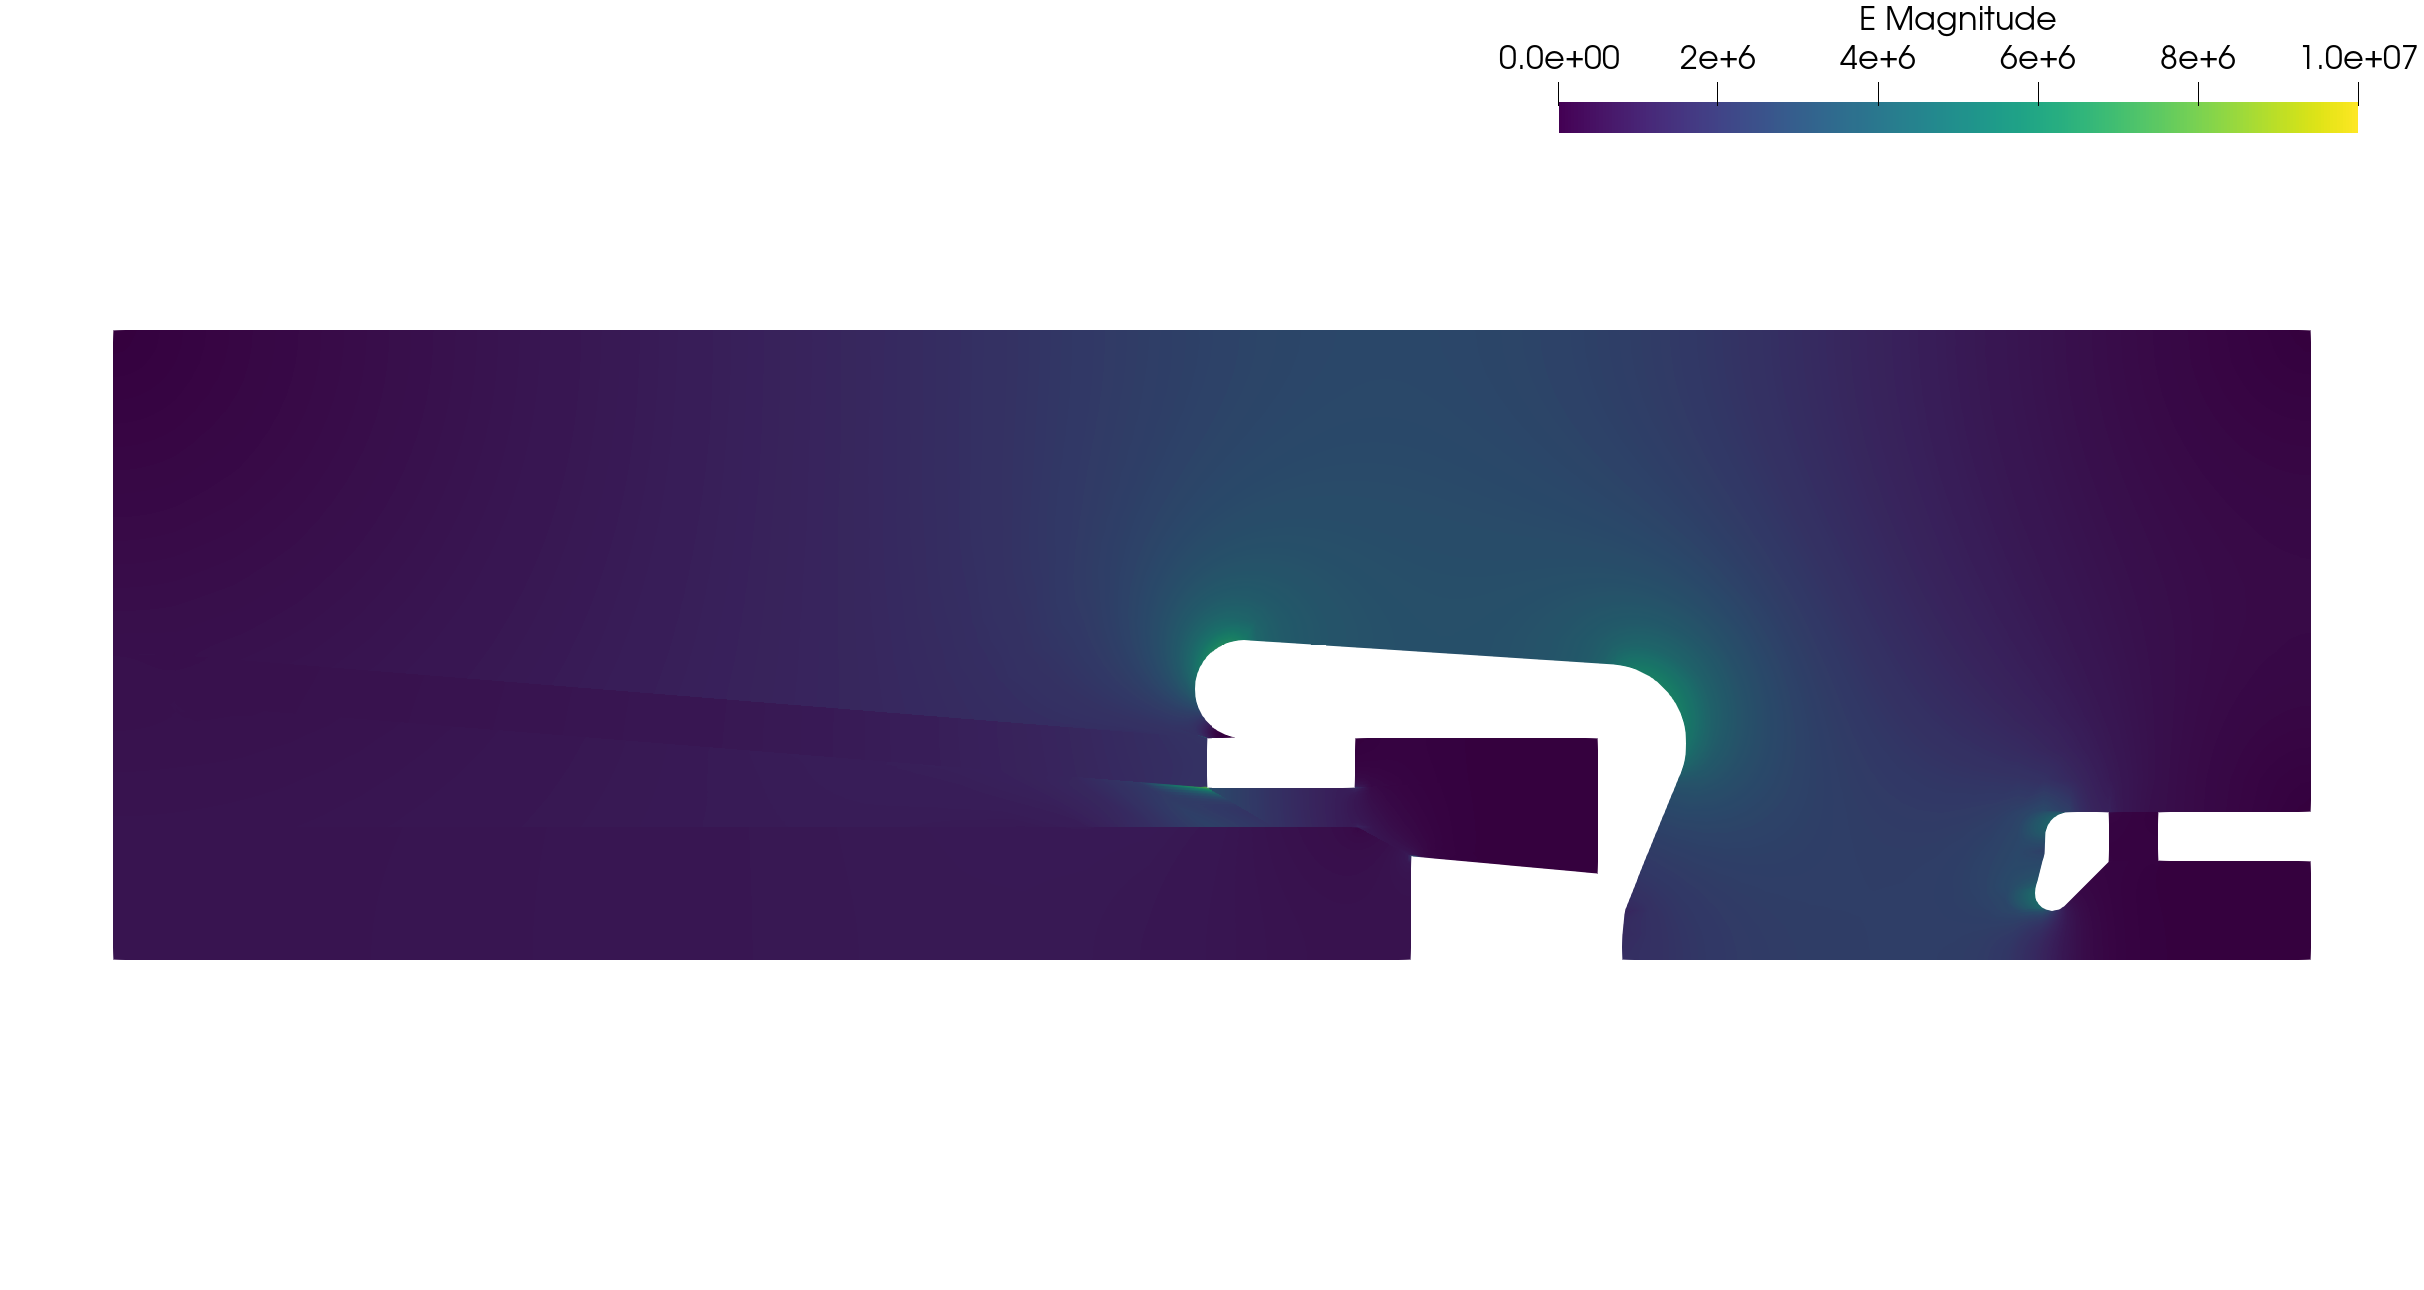
\includegraphics[width=\textwidth]{fig/200kV_v6}
      \caption{200kV.}
      \label{fig:200kV_v6}
   \end{subfigure}
   \begin{subfigure}{0.45\textwidth}
      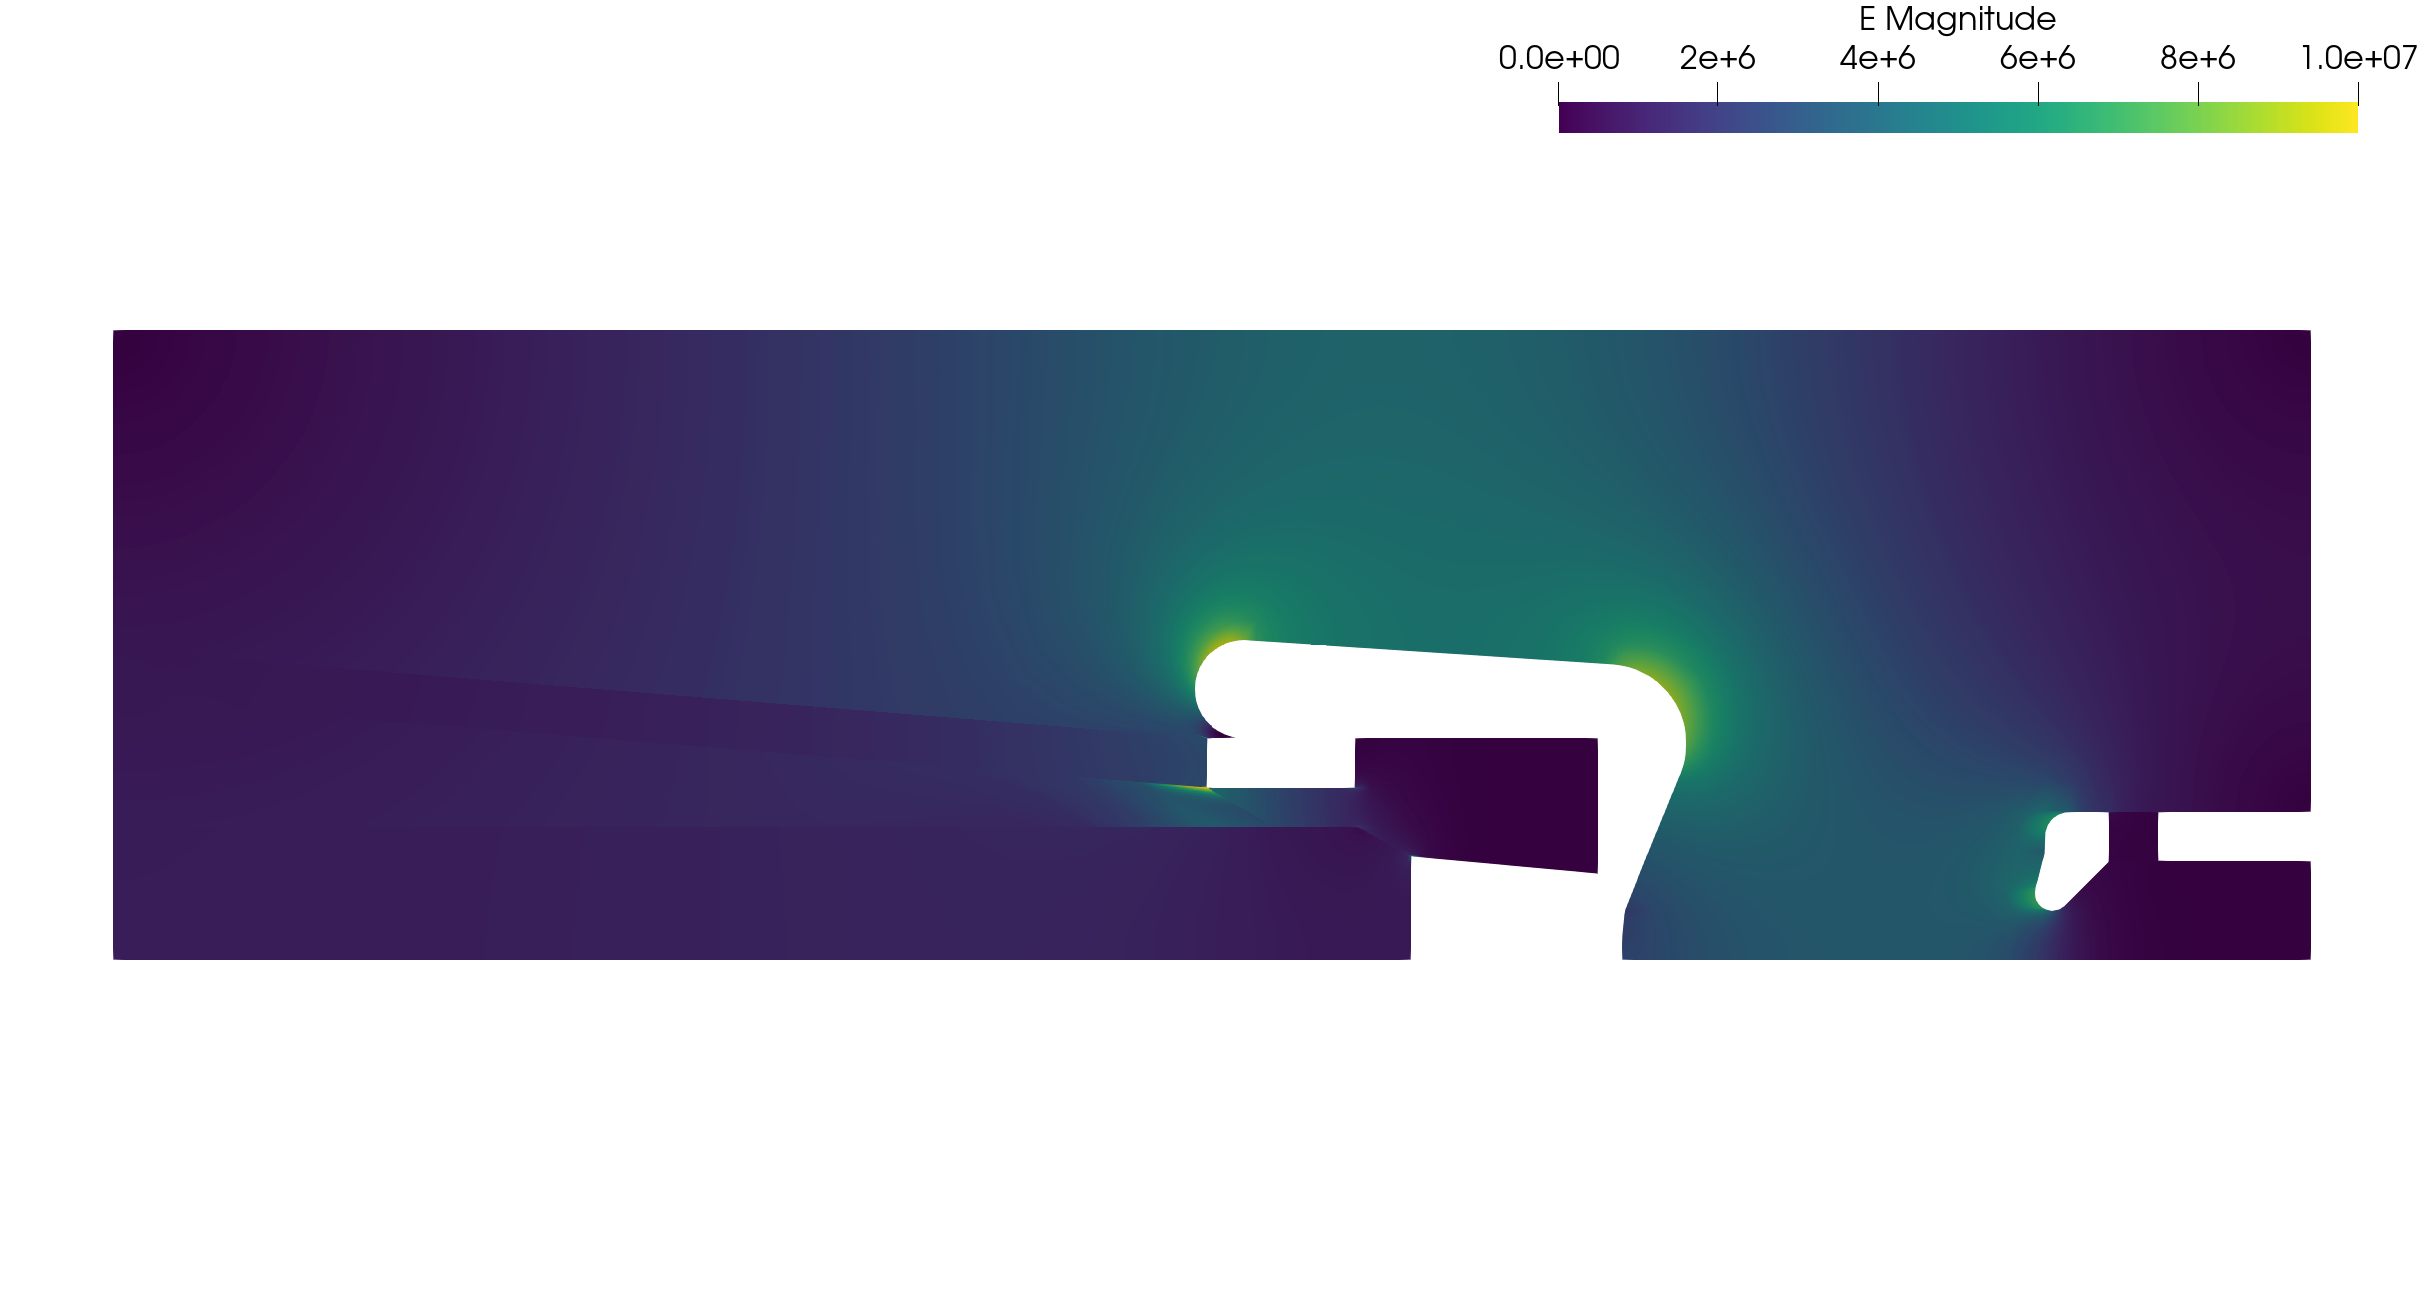
\includegraphics[width=\textwidth]{fig/300kV_v6}
      \caption{300kV.}
      \label{fig:300kV_v6}
   \end{subfigure}
\end{figure}
\end{center}

\subsection{Optimization}
The aim of the previous optimization was to minimize the maximal field amplitudes. The results are shown in fig.~\ref{fig:v5_opt}.

\begin{center}
\begin{figure}[H]
   \begin{subfigure}{0.45\textwidth}
      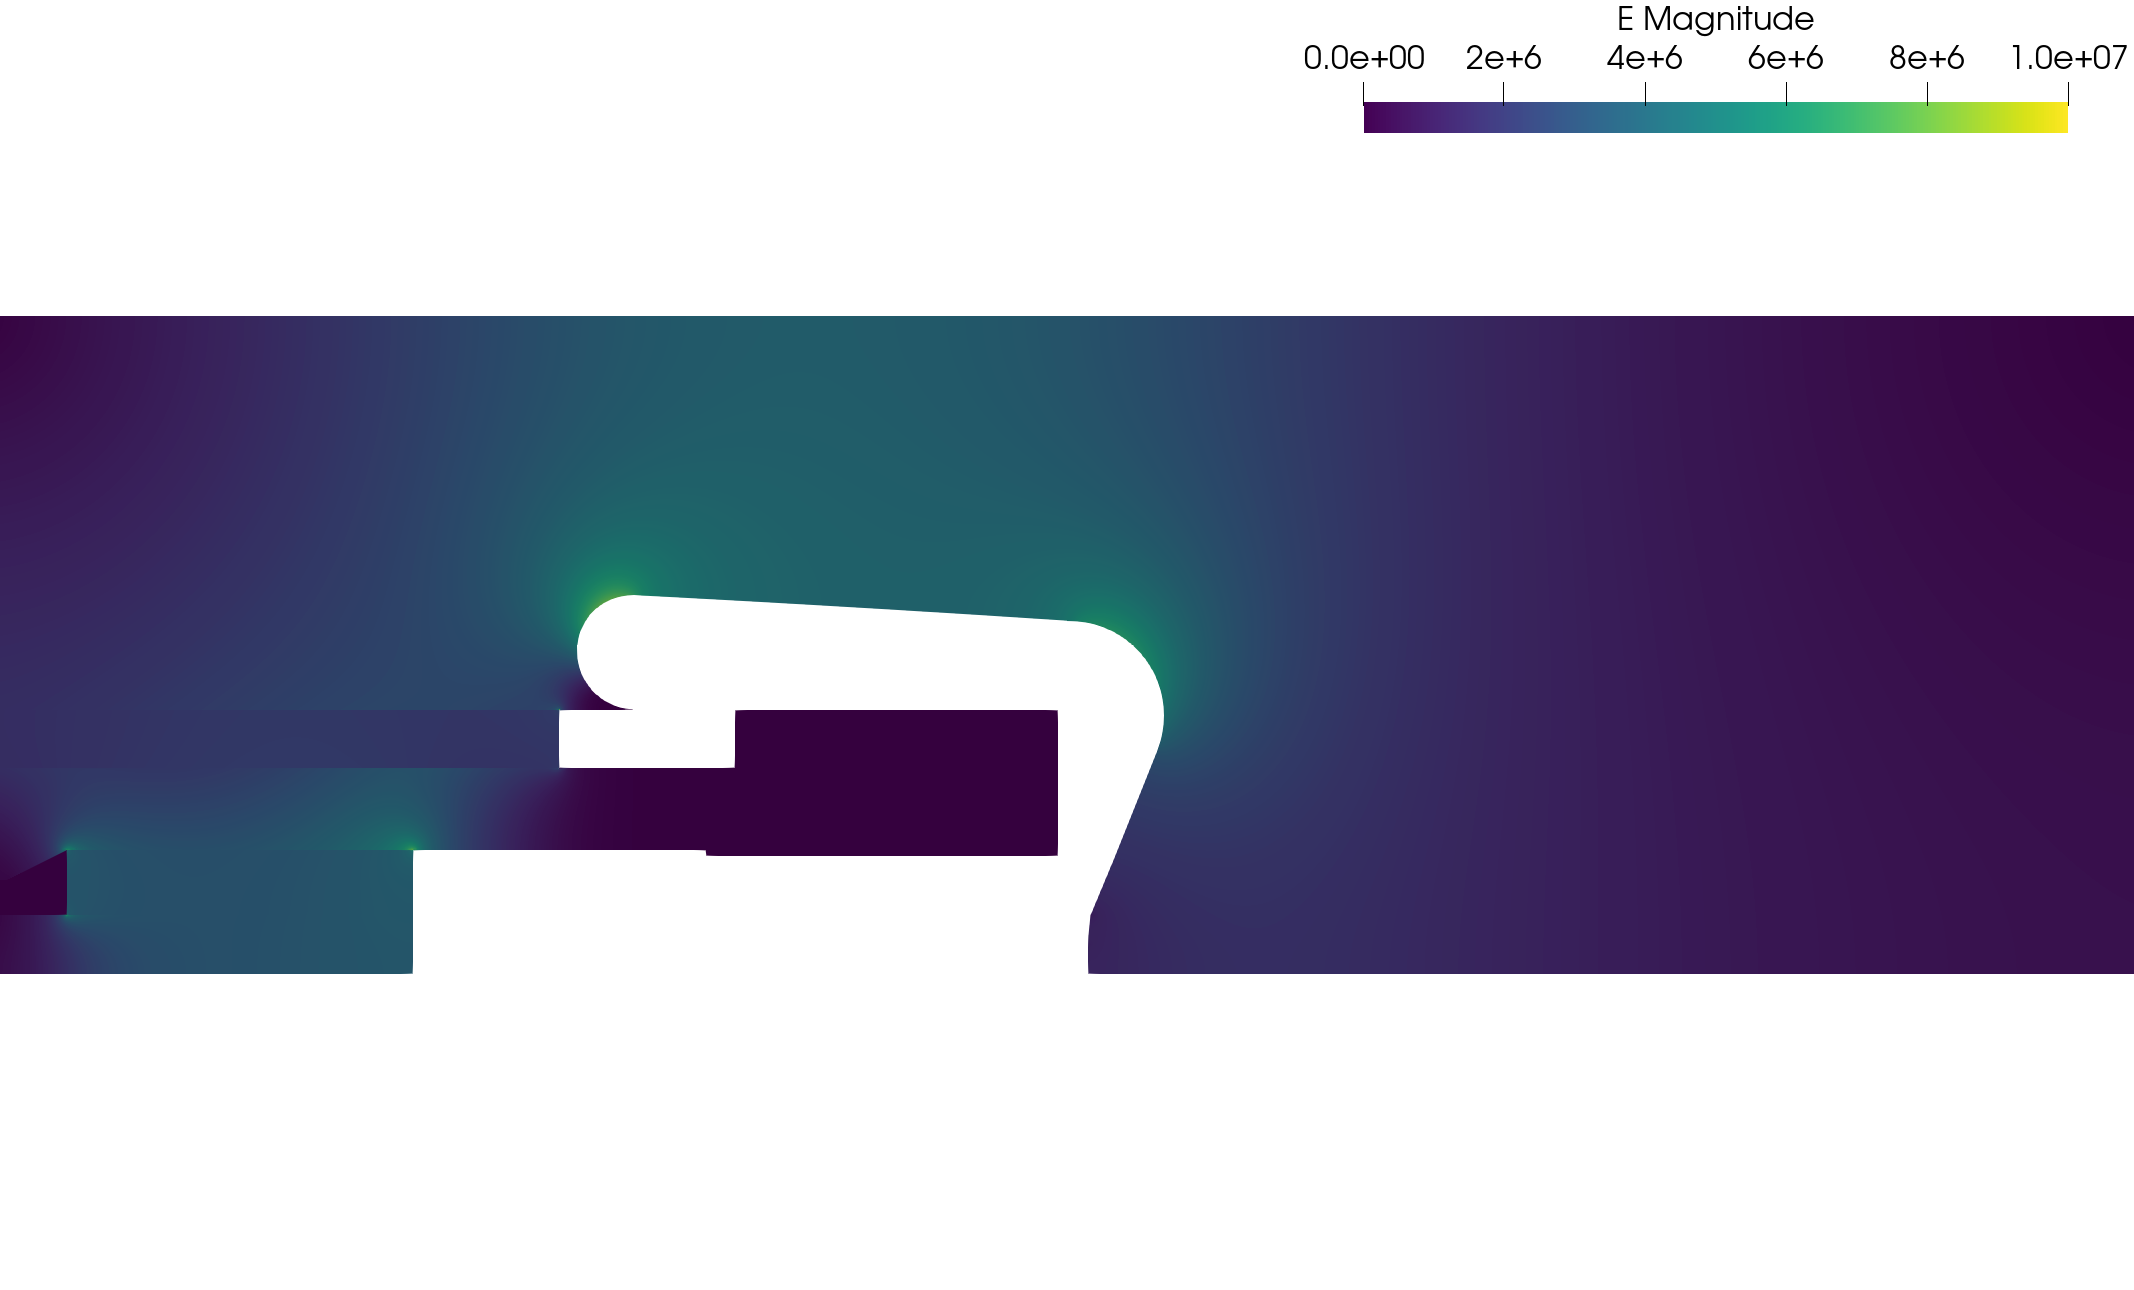
\includegraphics[width=\textwidth]{fig/v5_init}
      \caption{Version 5 initial solution.}
      \label{fig:v5_init}
   \end{subfigure}
   \begin{subfigure}{0.45\textwidth}
      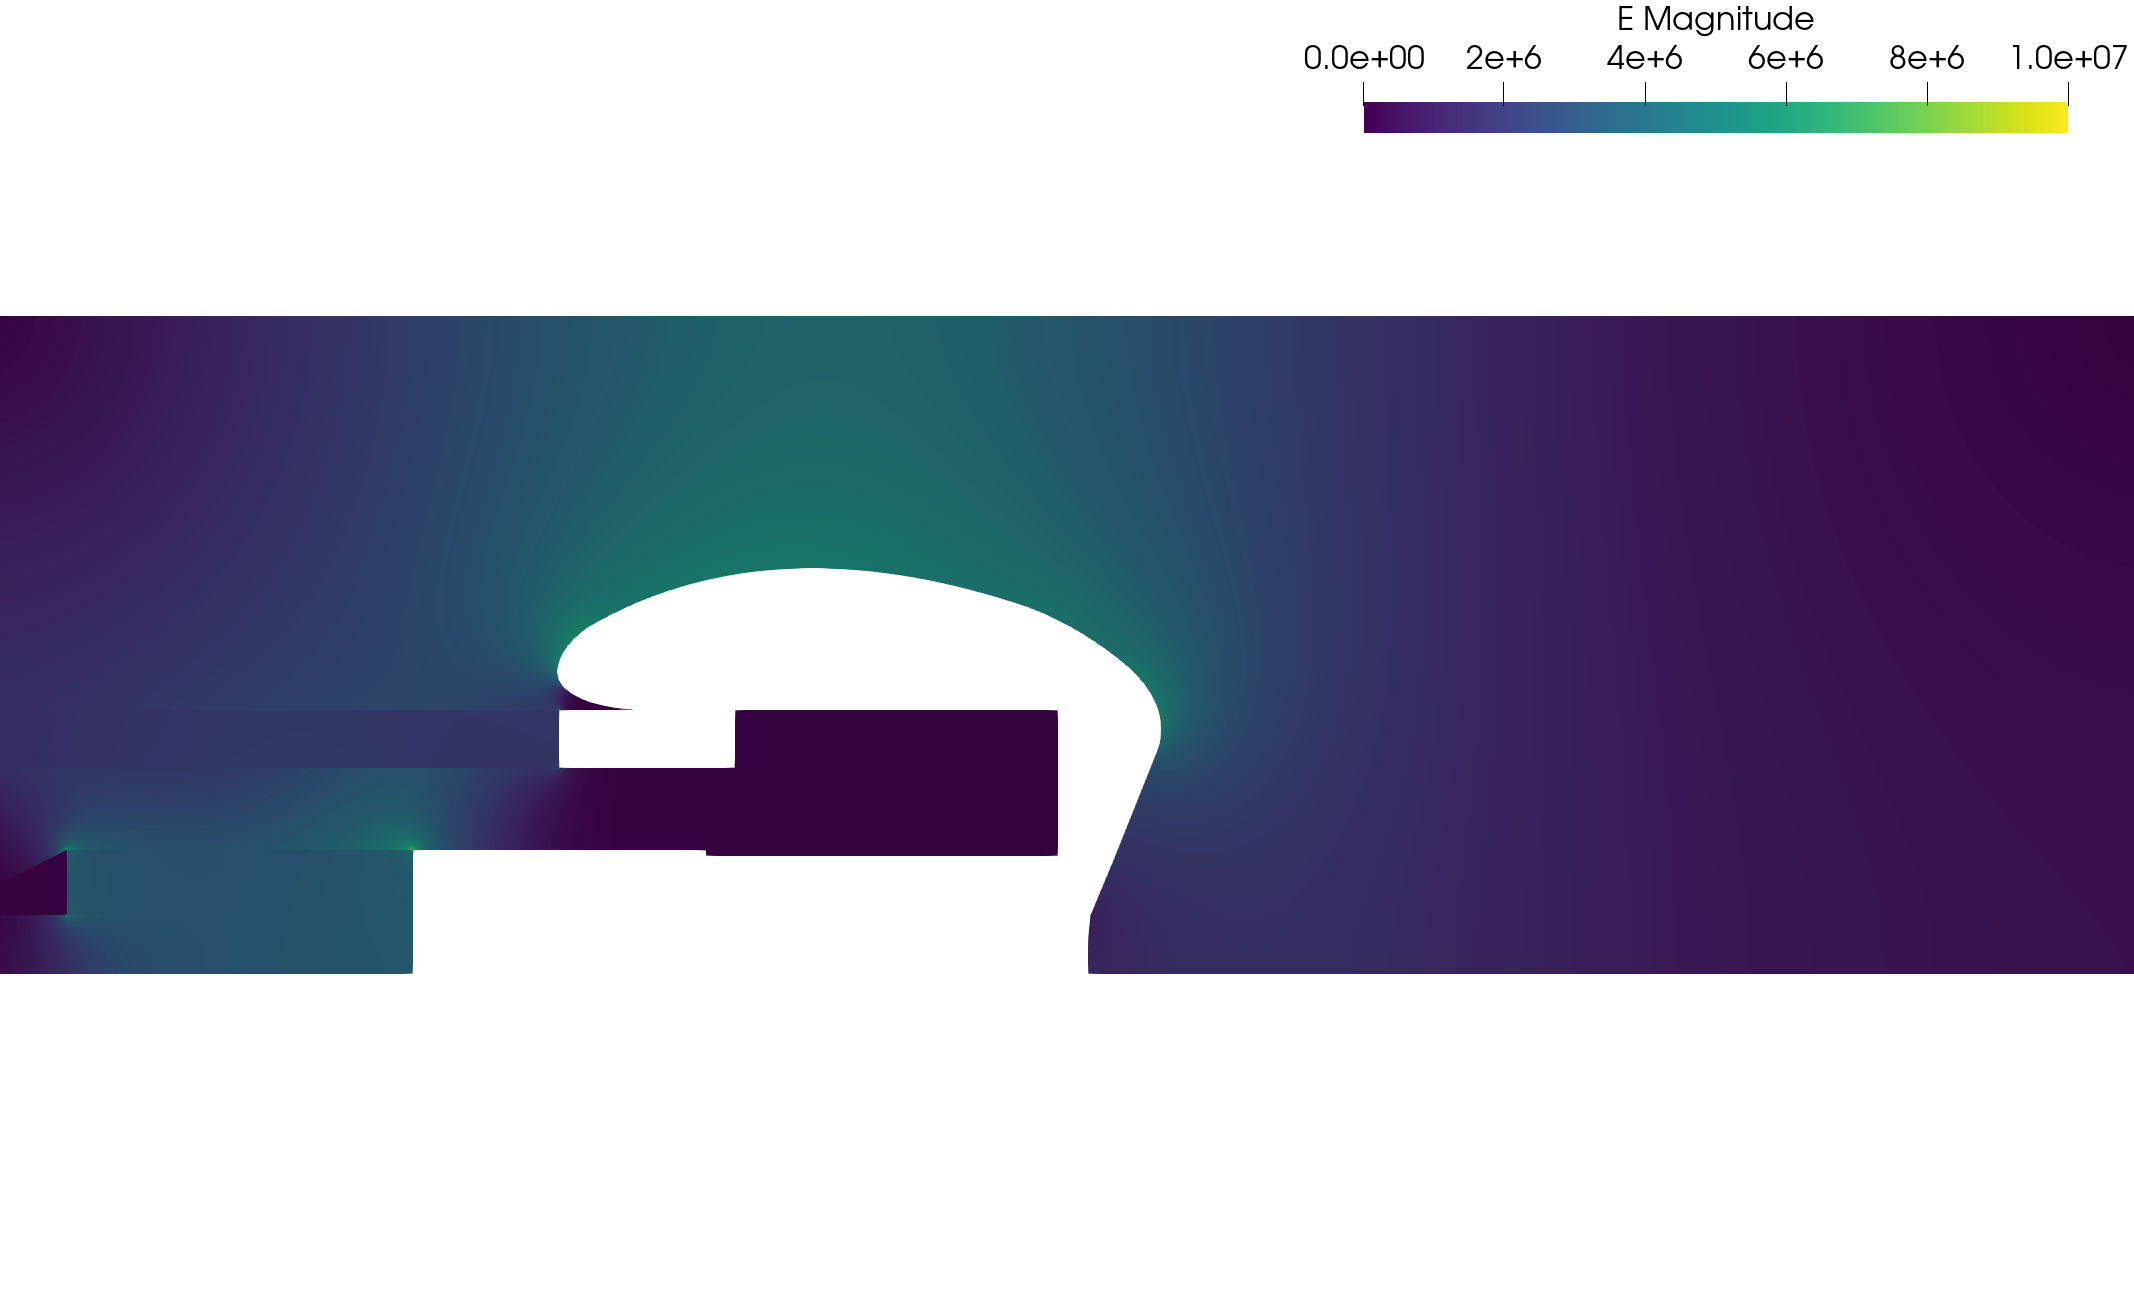
\includegraphics[width=\textwidth]{fig/v5_opt}
      \caption{Version 5 Optimization Result.}
      \label{fig:v5_opt}
   \end{subfigure}
\end{figure}
\end{center}

\subsection{Questions}
\begin{itemize}
   % \item \textbf{Geometry}: How much of patches 32,33,34,35 is insulator material or where does the metal start?\\

   \item \textbf{Optimization}: Also make size of patch 1,11 a parameter? (Anode voltage as well?)
   \item Is there a new maximal volume for electrode? (Otherwise we need to change the starting shape, since its volume is too large.)
   \item Is there a volume constraint for the anode ring?
   \item Optimize different parts of the geometry individually? (Couple by enforcing $C^1$ continuity at the curves interface.)
   \item Patches 8,9,10,14 for beam parameters, since 6,7 fixed? (Also anode ring.)\\

   \item \textbf{Astra}: Investigate fieldmap convergence. (Use fixed $H_\mathrm{max}$, field solution as in optimization, compare particle trajectories.) (Use specific norm?) (Only consider particles in cross-section?)
   \item Investigate time integrator convergence. (Use fixed fieldmap, $H_\mathrm{max}=H_\mathrm{min}$.)

   \item Use bunch length of 5 ps. (Uniform distribution?)
   \item Use laser spot size of 4 $\mathrm{mm}^2$. (Gaussian distribution with (2-5) $\sigma$ width of $2/\sqrt{\pi}$?)
   \item Other parameters: total charge 100 fC.

   \item Investigate convergence for number of probe particles and number of grid cells for 2D space charge. (Tracking is always 3D but 2D space charge computation respects mirror charges and should model the problem better?)

   \item \textbf{Cost Function} Use rms beam size, or individual trajectories (their minima). Other criteria?

   \item \textbf{General}: Let the constraint function return Inf in Lagrangian formulation or rather make all constraints be of similar magnitude? (Different solution: Use a vector for the ctrl-constraint.)\\
\end{itemize}

\subsection{Astra}
   \begin{center}
      \begin{figure}[H]
         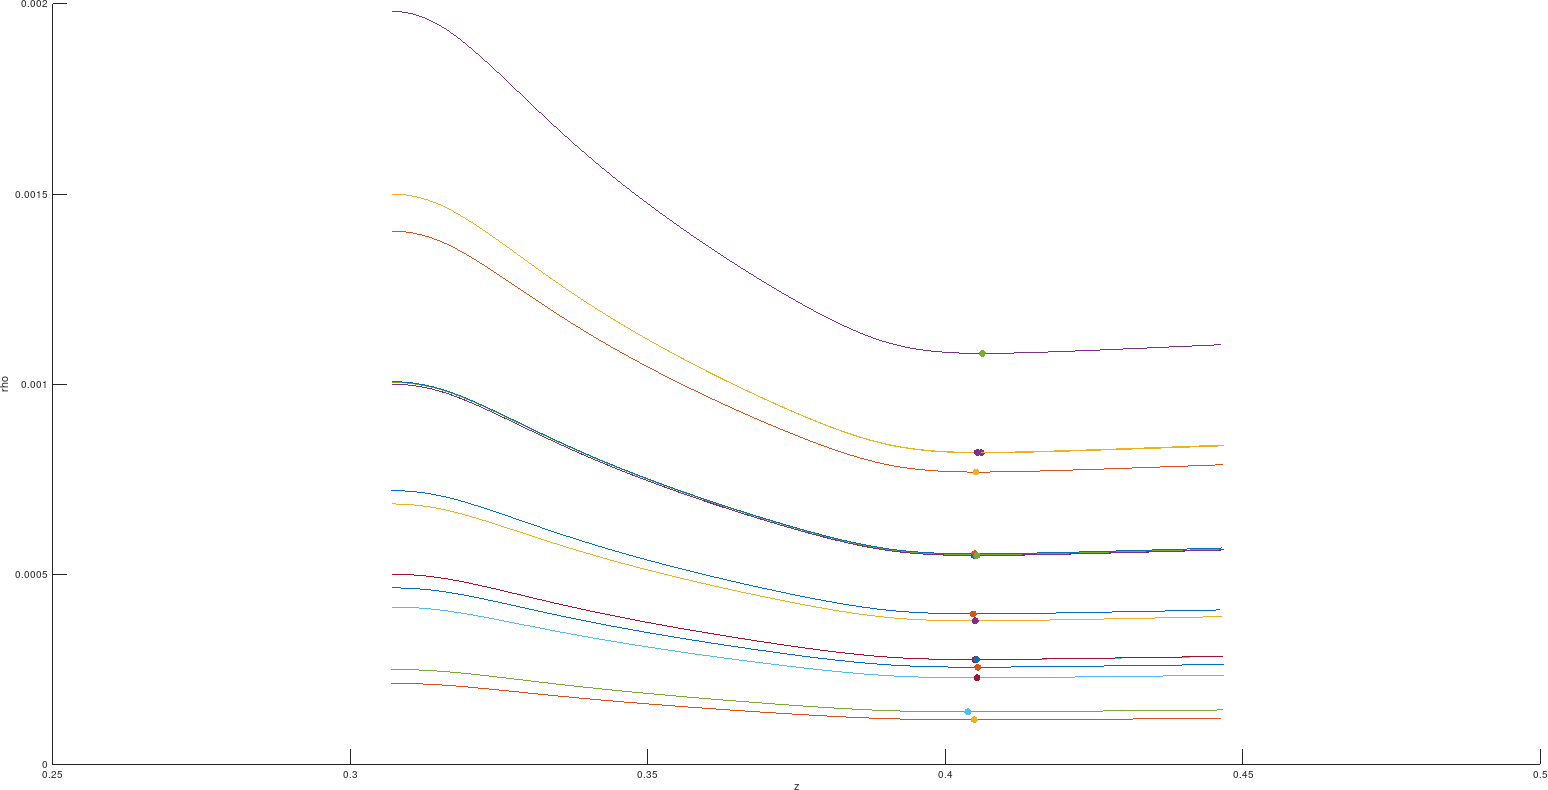
\includegraphics[width=\textwidth]{fig/astra}
      \end{figure}
   \end{center}
